\documentclass[12pt,a4paper]{article}

% ── Packages ─────────────────────────────────────────────────────────────────
\usepackage[T1]{fontenc}
\usepackage[utf8]{inputenc}
\usepackage[english]{babel}
\usepackage{lmodern}
\usepackage{microtype}
\usepackage{geometry}
\geometry{margin=2.5cm}
\usepackage{setspace}
\onehalfspacing

\usepackage{amsmath,amssymb}
\usepackage{graphicx}
\usepackage{float}
\usepackage{subcaption}
\usepackage{booktabs}
\usepackage{tabularx}
\usepackage{xcolor}
\usepackage{listings}
\usepackage{algorithm}
\usepackage{algpseudocode}
\usepackage{hyperref}
\hypersetup{
    colorlinks=true,
    linkcolor=blue!70!black,
    urlcolor=blue!70!black,
    citecolor=green!50!black,
}
\usepackage{caption}
\usepackage{enumitem}
\usepackage{fancyhdr}
\usepackage{titlesec}

% ── Code listing style ────────────────────────────────────────────────────────
\lstset{
    basicstyle=\ttfamily\small,
    keywordstyle=\color{blue!70!black}\bfseries,
    commentstyle=\color{gray},
    stringstyle=\color{green!50!black},
    breaklines=true,
    frame=single,
    framerule=0.4pt,
    rulecolor=\color{gray!40},
    backgroundcolor=\color{gray!5},
    numbers=left,
    numberstyle=\tiny\color{gray},
    numbersep=6pt,
    xleftmargin=12pt,
    captionpos=b,
}
\lstdefinelanguage{pseudocode}{
    morekeywords={FOR,IF,ELSE,THEN,DO,WHILE,RETURN,FUNCTION,INPUT,OUTPUT,END,TO,ALGORITHM,INITIALISE,BEGIN},
    sensitive=false,
    morecomment=[l]{//},
}

% ── Header / Footer ───────────────────────────────────────────────────────────
\pagestyle{fancy}
\fancyhf{}
\rhead{\small Genetic Algorithm — TSP \& CartPole-v1}
\lhead{\small Krupiński, Szczotka}
\cfoot{\thepage}
\renewcommand{\headrulewidth}{0.4pt}

% ── Graphics path ─────────────────────────────────────────────────────────────
% Paths are relative to the .tex file location (report_latex/)
\graphicspath{{../results/}{../docs/}{../results/task1/}{../results/task2/}{../results/task2/initial/}{../results/task2/trained/}{../results/task2/comparison/}}
\setlength{\headheight}{14pt}
\addtolength{\topmargin}{-2pt}

% ── Title ─────────────────────────────────────────────────────────────────────
\title{
    \vspace{-1cm}
    {\Large Biologically-Inspired Artificial Intelligence}\\[0.4em]
    {\LARGE\bfseries Genetic Algorithm for the Travelling Salesman Problem and CartPole-v1 Control}\\[0.6em]
    {\large BIAI Course Project Report}
}
\author{
    \textbf{Piotr Krupiński} \and \textbf{Jeremi Szczotka}\\[0.3em]
    \small Politechnika Śląska, Faculty of Automatic Control, Electronics and Computer Science
}
\date{\small June 2026}

% ─────────────────────────────────────────────────────────────────────────────
\begin{document}

\maketitle
\thispagestyle{empty}

\begin{abstract}
This report describes the design and implementation of a genetic algorithm (GA) framework applied to two distinct optimisation problems: the Travelling Salesman Problem (TSP) and the CartPole-v1 control task from the Gymnasium environment. The implementation uses a modular plugin architecture in which all domain-specific logic — population initialisation, fitness evaluation, crossover, mutation, and selection — is injected into a generic \texttt{GeneticAlgorithm} class as callable objects, requiring zero changes to the core loop when a new problem is introduced. For TSP, the GA achieves a route distance of~3.43 for 20~cities (within~10\% of the theoretical optimum of~3.1). For CartPole-v1, the algorithm discovers a working linear control policy in as few as~10 generations, achieving the maximum possible episode reward of~500. The report presents the theoretical background, full pseudocode, implementation details, experimental results, and hyperparameter analyses for both tasks.
\end{abstract}

\tableofcontents
\newpage

% ─────────────────────────────────────────────────────────────────────────────
\section{Introduction}
\label{sec:intro}
% ─────────────────────────────────────────────────────────────────────────────

Genetic algorithms are a class of metaheuristic optimisation methods inspired by the process of natural selection in biological evolution. Introduced by Holland~\cite{holland1975} and popularised by Goldberg~\cite{goldberg1989}, they operate on a population of candidate solutions (individuals), iteratively improving quality through selection of fit parents, recombination of their genetic material (crossover), and random perturbation (mutation).

This project was developed as part of the BIAI (Biologically-Inspired Artificial Intelligence) course at Politechnika Śląska. The primary objectives were:

\begin{enumerate}
    \item Implement a \textbf{generic, reusable GA framework} capable of solving different classes of problem without modifying the core loop.
    \item Apply the framework to the \textbf{Travelling Salesman Problem} (a classic combinatorial optimisation benchmark) and to the \textbf{CartPole-v1} environment (a continuous control task).
    \item Conduct \textbf{hyperparameter experiments} comparing operators and population sizes.
    \item Demonstrate the before-and-after improvement with graphical visualisations.
\end{enumerate}

Both problems were chosen deliberately because they require fundamentally different chromosome representations (discrete permutations vs. continuous real-valued vectors) and different genetic operators, making them an ideal test of the framework's generality.

The complete source code is available at \url{https://github.com/piotrek1459/biai-genetic-cartpole}.

% ─────────────────────────────────────────────────────────────────────────────
\section{Genetic Algorithms — Theory}
\label{sec:theory}
% ─────────────────────────────────────────────────────────────────────────────

\subsection{Biological Analogy}

A genetic algorithm models a population of organisms competing for survival in an environment. Individuals with higher fitness (closer to the optimal solution) are more likely to reproduce. Over many generations, beneficial traits spread through the population and the average quality improves.

\subsection{Algorithm Components}

\paragraph{Chromosome (individual).}
A chromosome encodes one candidate solution. The representation depends entirely on the problem:
\begin{itemize}
    \item For combinatorial problems (TSP), a chromosome is a permutation of integer indices.
    \item For continuous optimisation (CartPole), a chromosome is a vector of real numbers.
\end{itemize}

\paragraph{Fitness function.}
Maps each chromosome to a scalar quality score. \emph{Higher is always better} in this implementation — minimisation problems (TSP distance) are inverted to become maximisation problems.

\paragraph{Selection.}
Determines which individuals become parents. Two strategies are implemented:
\begin{description}
    \item[Tournament selection] Randomly draw $k$ individuals, select the one with the highest fitness. Repeat $n_\text{select}$ times. Higher $k$ means stronger selection pressure.
    \item[Roulette-wheel selection] Assign each individual a selection probability proportional to its fitness: $p_i = f_i / \sum_j f_j$.
\end{description}

\paragraph{Crossover (recombination).}
Combines genetic material from two parents to produce two offspring. The operator must be \emph{representation-aware}: permutation crossover must not create duplicate or missing genes.

\paragraph{Mutation.}
Introduces random variation to maintain population diversity and explore new regions of the search space. The mutation rate controls how frequently an individual is perturbed.

\paragraph{Elitism.}
The top $n_\text{elite}$ individuals are copied unchanged into the next generation. This prevents the loss of the best solution found so far.

\subsection{Full Pseudocode}

Algorithm~\ref{alg:ga} presents the complete pseudocode of the implemented GA.

\begin{algorithm}[H]
\caption{GeneticAlgorithm.run()}
\label{alg:ga}
\begin{algorithmic}[1]
\Require $\textit{init\_fn}, \textit{fitness\_fn}, \textit{crossover\_fn}, \textit{mutation\_fn}, \textit{selection\_fn}, \textit{config}$
\State $\textit{population} \leftarrow \textit{init\_fn}(\textit{config})$
\State $\textit{best\_so\_far} \leftarrow -\infty$; \; $\textit{stagnation} \leftarrow 0$
\For{$\textit{gen} = 0$ \textbf{to} $n_\text{generations} - 1$}
    \State $\textit{fitness}[i] \leftarrow \textit{fitness\_fn}(\textit{population}[i])$ \quad (parallel if $n_\text{jobs} \neq 1$)
    \State $\textit{history\_best}.\text{append}(\max(\textit{fitness}))$; \; $\textit{history\_avg}.\text{append}(\text{mean}(\textit{fitness}))$
    \If{$\max(\textit{fitness}) > \textit{best\_so\_far} + \varepsilon$}
        \State $\textit{best\_so\_far} \leftarrow \max(\textit{fitness})$; \; $\textit{stagnation} \leftarrow 0$; \; $\textit{boost} \leftarrow \textbf{False}$
    \Else
        \State $\textit{stagnation} \leftarrow \textit{stagnation} + 1$
        \State $\textit{boost} \leftarrow (\textit{stagnation} \geq \textit{patience})$
        \If{$\textit{boost}$} \; $\textit{stagnation} \leftarrow 0$ \EndIf
    \EndIf
    \State $\textit{elites} \leftarrow$ top $n_\text{elite}$ individuals (unchanged)
    \State $\textit{parents} \leftarrow \textit{selection\_fn}(\textit{population}, \textit{fitness},\; n_\text{pop} - n_\text{elite})$
    \State $\textit{offspring} \leftarrow [\;]$
    \For{$i = 0, 2, 4, \ldots$}
        \State $(c_1, c_2) \leftarrow \textit{crossover\_fn}(\textit{parents}[i],\; \textit{parents}[i{+}1])$
        \State $c_1 \leftarrow \textit{mutation\_fn}(c_1)$; \; $c_2 \leftarrow \textit{mutation\_fn}(c_2)$
        \If{$\textit{boost}$} \; $c_1 \leftarrow \textit{mutation\_fn}(c_1)$; \; $c_2 \leftarrow \textit{mutation\_fn}(c_2)$ \EndIf
        \State $\textit{offspring}.\text{append}(c_1, c_2)$
    \EndFor
    \State $\textit{population} \leftarrow \textit{elites} \cup \textit{offspring}[0 : n_\text{pop} - n_\text{elite}]$
\EndFor
\State \Return $\{\textit{best}, \textit{best\_fitness}, \textit{history\_best}, \textit{history\_avg}, \textit{stagnation\_events}\}$
\end{algorithmic}
\end{algorithm}

% ─────────────────────────────────────────────────────────────────────────────
\section{Implementation Architecture}
\label{sec:arch}
% ─────────────────────────────────────────────────────────────────────────────

\subsection{Plugin Interface}

The central design decision was to make the \texttt{GeneticAlgorithm} class completely generic through \emph{dependency injection}. In Python, functions are first-class objects — they can be assigned to variables and passed as arguments. The constructor stores the five operator callables as instance attributes:

\begin{lstlisting}[language=Python, caption={GeneticAlgorithm constructor (ga\_base.py)}]
class GeneticAlgorithm:
    def __init__(self, config, init_fn, fitness_fn,
                 crossover_fn, mutation_fn, selection_fn):
        self.config       = config
        self.init_fn      = init_fn
        self.fitness_fn   = fitness_fn
        self.crossover_fn = crossover_fn
        self.mutation_fn  = mutation_fn
        self.selection_fn = selection_fn
\end{lstlisting}

The evolution loop calls these attributes without knowing their domain:

\begin{lstlisting}[language=Python, caption={Generic calls inside run() and \_breed()}]
population = self.init_fn(self.config)          # once at start
fitness[i] = self.fitness_fn(population[i])     # every individual
parents    = self.selection_fn(pop, fit, n)     # every generation
c1, c2     = self.crossover_fn(p1, p2)          # every pair
c1         = self.mutation_fn(c1)               # every offspring
\end{lstlisting}

To add a new problem (Task N), the developer needs only to implement these five functions and pass them to the constructor. The \texttt{ga\_base.py} file requires no modification.

\subsection{Module Structure}

Table~\ref{tab:modules} summarises the module organisation.

\begin{table}[H]
\centering
\caption{Module structure and responsibilities}
\label{tab:modules}
\begin{tabularx}{\textwidth}{llX}
\toprule
\textbf{File} & \textbf{Module} & \textbf{Responsibility} \\
\midrule
\texttt{src/common/ga\_base.py} & common & Generic GA loop; no domain knowledge \\
\texttt{src/common/selection.py} & common & \texttt{tournament\_selection}, \texttt{roulette\_selection} \\
\texttt{src/common/crossover.py} & common & OX, PMX (permutation); uniform, arithmetic (real) \\
\texttt{src/common/mutation.py} & common & swap, inversion, scramble (permutation); gaussian (real) \\
\texttt{src/task1\_tsp/tsp\_ga.py} & task1 & TSP entry point; city generation; fitness closure \\
\texttt{src/task1\_tsp/visualization.py} & task1 & Fitness history plot (dual-axis); route visualisation \\
\texttt{src/task1\_tsp/experiments.py} & task1 & Hyperparameter sweep scripts \\
\texttt{src/task2\_cartpole/cartpole\_policy.py} & task2 & \texttt{LinearPolicy}; \texttt{evaluate\_policy\_with\_stats} \\
\texttt{src/task2\_cartpole/train\_ga.py} & task2 & CartPole entry point; episode recording; comparison video \\
\texttt{src/task2\_cartpole/visualization.py} & task2 & Reward history; control performance; comparison plots \\
\bottomrule
\end{tabularx}
\end{table}

\subsection{Five Callables — Signatures}

\begin{table}[H]
\centering
\caption{The five plugin callables}
\label{tab:callables}
\begin{tabularx}{\textwidth}{llX}
\toprule
\textbf{Callable} & \textbf{Signature} & \textbf{Returns} \\
\midrule
\texttt{init\_fn} & \texttt{(config) -> list[ndarray]} & Initial population of \texttt{pop\_size} chromosomes \\
\texttt{fitness\_fn} & \texttt{(individual) -> float} & Fitness score; higher is always better \\
\texttt{crossover\_fn} & \texttt{(p1, p2) -> (c1, c2)} & Two children derived from two parents \\
\texttt{mutation\_fn} & \texttt{(individual) -> ndarray} & Mutated copy of the input individual \\
\texttt{selection\_fn} & \texttt{(pop, fit, n) -> list} & $n$ parents selected from the population \\
\bottomrule
\end{tabularx}
\end{table}

\subsection{Parallel Evaluation}

Fitness evaluation is parallelised using \texttt{concurrent.futures.ThreadPoolExecutor}. When \texttt{n\_jobs~=~-1}, all available CPU threads are used. This is particularly beneficial for CartPole, where each fitness call runs five independent Gymnasium episodes ($\approx 2{,}500$ environment steps per individual).

\subsection{Adaptive Mutation}

A stagnation counter tracks how many consecutive generations pass without fitness improvement. When the counter exceeds \texttt{adaptive\_patience} (25 for TSP, 15 for CartPole), the mutation operator is applied \emph{twice} per offspring for that generation (the ``boost''). This mechanism is inspired by the exploration–exploitation trade-off in reinforcement learning: when the reward signal flatlines, the agent increases exploration.

% ─────────────────────────────────────────────────────────────────────────────
\section{Task 1: Travelling Salesman Problem}
\label{sec:tsp}
% ─────────────────────────────────────────────────────────────────────────────

\subsection{Problem Definition}

Given $n$ cities with known coordinates, find the shortest Hamiltonian cycle — a tour that visits every city exactly once and returns to the starting city. The decision version of TSP is NP-complete; the optimisation version is NP-hard. For $n = 20$ random cities in the unit square, the theoretical expected optimum is approximately $0.7\sqrt{n} \approx 3.1$.

\subsection{Chromosome Representation}

A chromosome is a permutation of city indices $\{0, 1, \ldots, n{-}1\}$, e.g. $[2, 0, 4, 1, 3]$ represents the route city~2 $\to$ city~0 $\to$ city~4 $\to$ city~1 $\to$ city~3 $\to$ city~2. The length-$n$ array always contains each index exactly once; all genetic operators must preserve this property.

\subsection{Fitness Function}

The fitness is the inverse of the total round-trip Euclidean distance, augmented by a path-balance (smoothness) bonus:

\begin{equation}
f(\sigma) = \frac{1}{d(\sigma) + \varepsilon} \times \left(1 + w_s \cdot \frac{1}{1 + \mathrm{CV}(\sigma)}\right)
\label{eq:tsp_fitness}
\end{equation}

where $d(\sigma) = \sum_{i=0}^{n-2} \|\mathbf{c}_{\sigma(i+1)} - \mathbf{c}_{\sigma(i)}\| + \|\mathbf{c}_{\sigma(0)} - \mathbf{c}_{\sigma(n-1)}\|$ is the total distance, $\varepsilon = 10^{-6}$ prevents division by zero, $\mathrm{CV}(\sigma) = \sigma_l / \mu_l$ is the coefficient of variation of segment lengths, and $w_s = 0.2$ weights the smoothness bonus. A perfectly balanced route (all segments equal length) achieves $\mathrm{CV} = 0$ and the maximum bonus of $1.2\times$.

\subsection{Genetic Operators}

\paragraph{Order Crossover (OX).}
A random segment $[a, b]$ is copied from parent $p_1$ into the child at the same positions. The remaining genes are filled from $p_2$ in order, starting at position $b$, wrapping around, skipping genes already present. OX preserves the \emph{relative order} of cities from $p_2$. This is the default operator.

\paragraph{Partially Mapped Crossover (PMX).}
Copies segment $[a, b]$ from $p_1$ and fills the rest from $p_2$, resolving conflicts by following the position-mapping defined by the segment. PMX preserves \emph{absolute positions}. Available as an alternative via CONFIG.

\paragraph{Inversion Mutation (default).}
A random sub-sequence is reversed. This is the strongest permutation mutation implemented: it can move cities far from their original positions while always producing a valid tour.

\paragraph{Swap Mutation.}
Two random genes are exchanged. Simpler and weaker than inversion; available for comparison.

\paragraph{Scramble Mutation.}
A random sub-sequence is shuffled. Useful when the population has lost diversity.

\subsection{Configuration}

\begin{table}[H]
\centering
\caption{Default TSP configuration}
\label{tab:tsp_config}
\begin{tabular}{lll}
\toprule
\textbf{Parameter} & \textbf{Value} & \textbf{Notes} \\
\midrule
$n_\text{cities}$ & 20 & Random points in $[0,1]^2$ \\
$n_\text{pop}$ & 80 & Good diversity without excessive runtime \\
$n_\text{gen}$ & 300 & Converges well before limit \\
$n_\text{elite}$ & 2 & Preserve best solutions \\
Crossover & OX & More stable than PMX on first run \\
Mutation & Inversion, rate=0.10 & Default; strong perturbation \\
Selection & Tournament, $k=4$ & Strong selection pressure \\
$w_s$ & 0.2 & Smoothness bonus weight \\
Adaptive patience & 25 & Generations without improvement before boost \\
\bottomrule
\end{tabular}
\end{table}

\subsection{Results}

Figure~\ref{fig:tsp_routes} shows the initial random route and the best route found after 300 generations.

\begin{figure}[H]
\centering
\begin{subfigure}[b]{0.47\textwidth}
    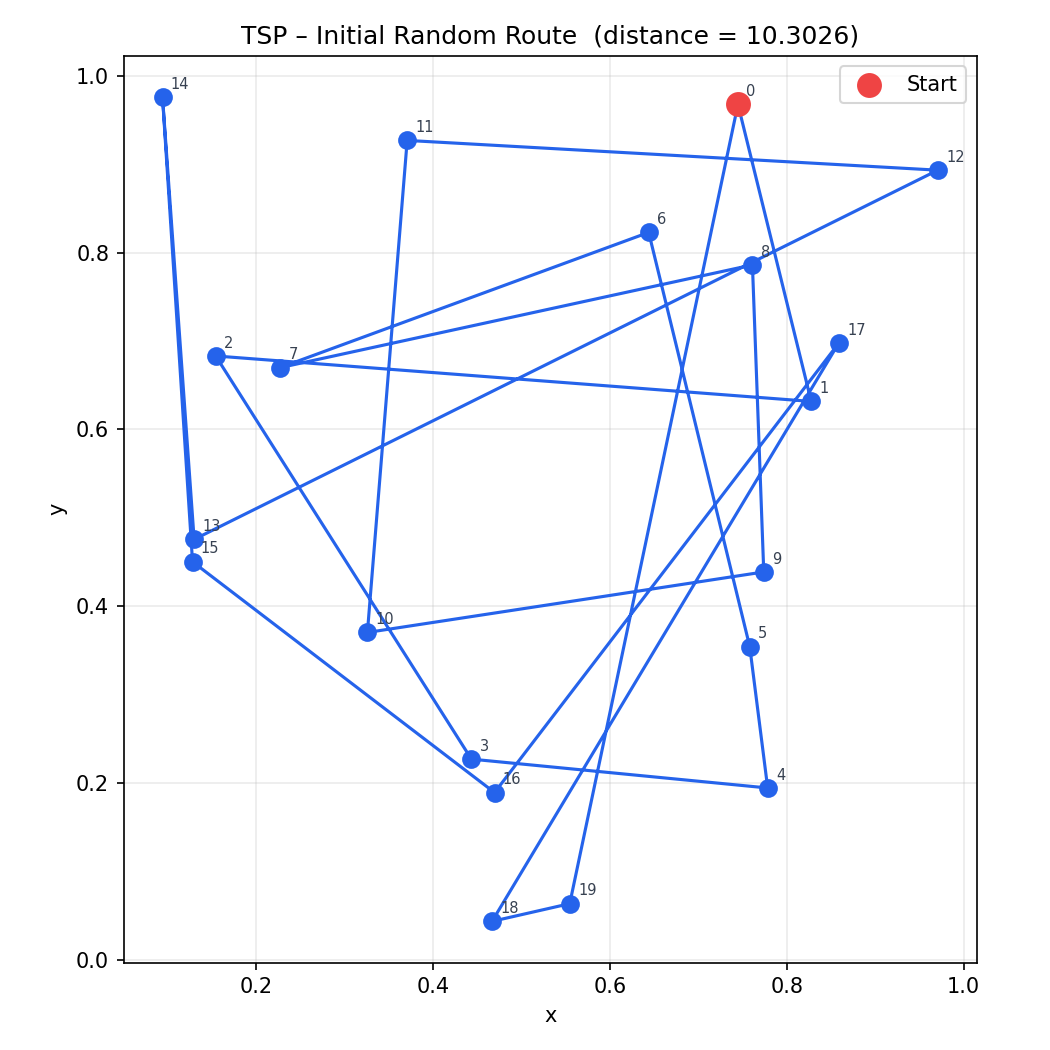
\includegraphics[width=\textwidth]{initial_route.png}
    \caption{Initial random route (distance $\approx$ 6--8)}
\end{subfigure}
\hfill
\begin{subfigure}[b]{0.47\textwidth}
    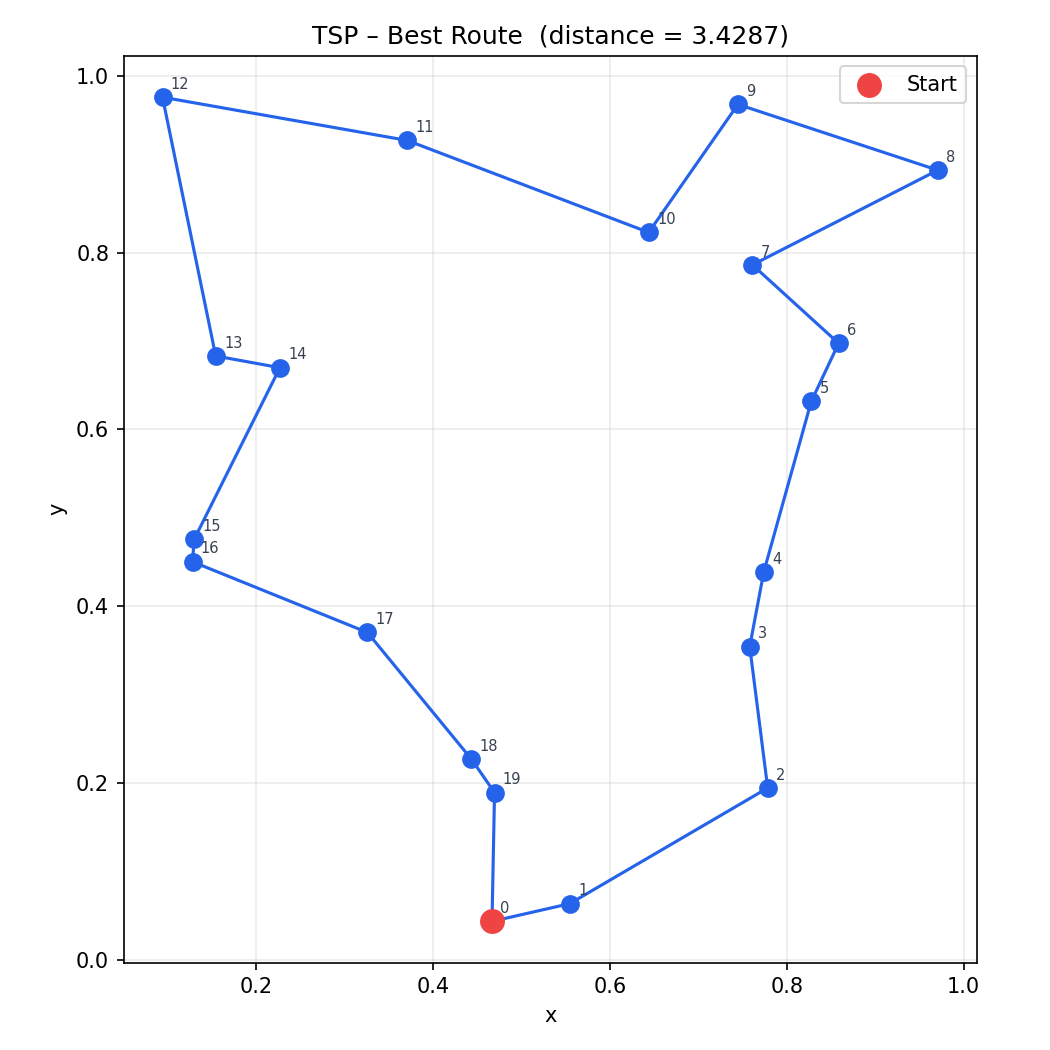
\includegraphics[width=\textwidth]{best_route.png}
    \caption{Best route after GA (distance = 3.43)}
\end{subfigure}
\caption{TSP: before and after GA optimisation}
\label{fig:tsp_routes}
\end{figure}

Figure~\ref{fig:tsp_history} shows the fitness and derived distance over generations. Fitness rises sharply in the first 50 generations, then stabilises. The dual-axis display makes the improvement directly readable in distance units without knowledge of the fitness formula.

\begin{figure}[H]
\centering

\includegraphics[width=0.78\textwidth]{fitness_history.png}
\caption{TSP fitness and route distance over 300 generations. Left axis: fitness $= 1/d$. Right axis: distance (inverted scale). Dotted vertical lines mark adaptive boost events.}
\label{fig:tsp_history}
\end{figure}

\subsection{Hyperparameter Experiments}

\subsubsection{Operator Comparison}

Figure~\ref{fig:tsp_operators} compares four operator combinations across 200 generations.

\begin{figure}[H]
\centering
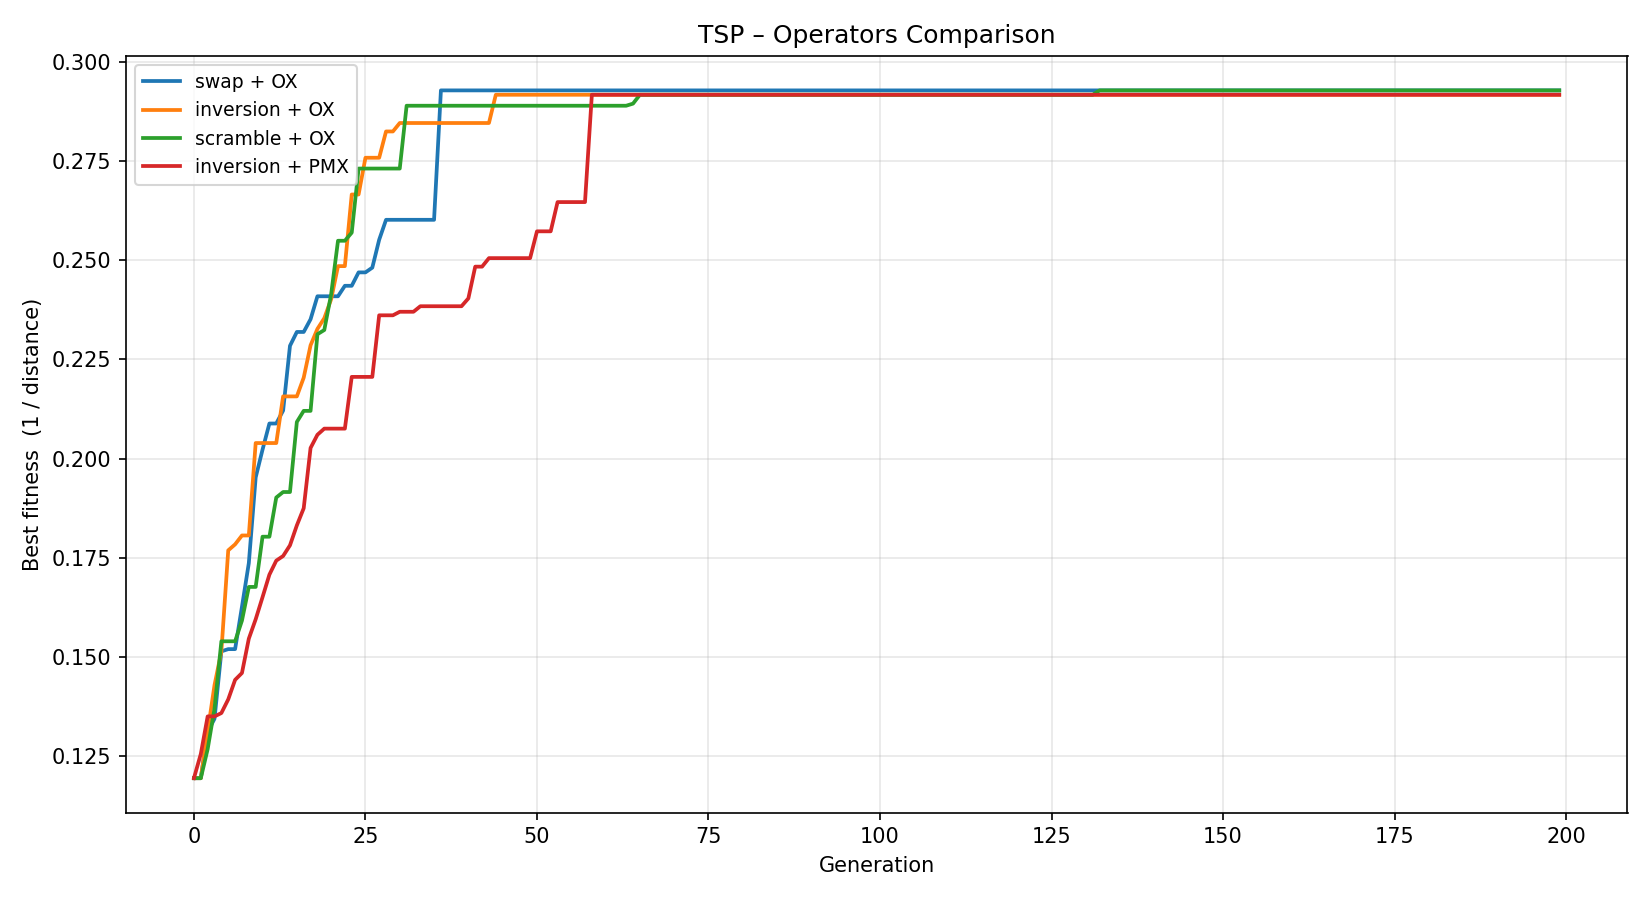
\includegraphics[width=0.80\textwidth]{comparison_operators.png}
\caption{TSP operator comparison: all combinations reach similar final quality. Inversion+OX converges most consistently.}
\label{fig:tsp_operators}
\end{figure}

All four configurations reach a final fitness within 2\% of each other, suggesting that the algorithm is robust to operator choice on this problem size. Inversion mutation outperforms swap because it introduces larger perturbations; OX and PMX produce similar results because the route's relative city ordering is more important than absolute positions for 20-city instances.

\subsubsection{Population Size Comparison}

Figure~\ref{fig:tsp_pop} compares population sizes of 40, 80, and 160.

\begin{figure}[H]
\centering

\includegraphics[width=0.80\textwidth]{comparison_population_size.png}
\caption{TSP population size comparison: larger populations provide smoother convergence but similar final quality.}
\label{fig:tsp_pop}
\end{figure}

All three population sizes converge to similar final fitness values for 20 cities. Larger populations provide more stable convergence curves and are less susceptible to premature convergence, at the cost of more fitness evaluations per generation.

% ─────────────────────────────────────────────────────────────────────────────
\section{Task 2: CartPole-v1}
\label{sec:cartpole}
% ─────────────────────────────────────────────────────────────────────────────

\subsection{Environment}

CartPole-v1 is a classic control benchmark from the Gymnasium library~\cite{gymnasium2023}. A pole is attached by a pivot to a cart moving along a frictionless track. The agent must keep the pole balanced by applying a force to the left or right at each discrete time step. The observation vector is:

\begin{equation}
\mathbf{o} = [\underbrace{x}_{\text{cart position}},\; \underbrace{\dot{x}}_{\text{cart velocity}},\; \underbrace{\theta}_{\text{pole angle}},\; \underbrace{\dot{\theta}}_{\text{angular velocity}}]
\label{eq:observation}
\end{equation}

The episode terminates when $|x| > 2.4$, $|\theta| > 12^{\circ}$, or 500 steps have elapsed. The reward is $+1$ for every step the pole remains balanced, so the maximum episode reward is 500.

\subsection{Chromosome and Linear Policy}

The chromosome is a vector of 5 real numbers $\mathbf{w} = [w_0, w_1, w_2, w_3, b]$ representing weights and a bias for a linear controller:

\begin{equation}
\text{action} = \begin{cases}
1 & \text{if } w_0 x + w_1 \dot{x} + w_2 \theta + w_3 \dot{\theta} + b > 0 \\
0 & \text{otherwise}
\end{cases}
\label{eq:policy}
\end{equation}

CartPole-v1 is linearly stabilisable — there exists a classical LQR solution~\cite{ogata2010}. The GA can discover a linear policy without any knowledge of the system's dynamics.

\subsection{Fitness Function}

Because the initial observation is randomised at each episode reset, a single episode evaluation is noisy. To reduce variance, each individual is evaluated over $n_\text{eval} = 5$ independent episodes, and the fitness incorporates a stability penalty:

\begin{equation}
f(\mathbf{w}) = \bar{r}(\mathbf{w}) - \lambda \cdot \sigma_r(\mathbf{w})
\label{eq:cartpole_fitness}
\end{equation}

where $\bar{r}$ is the mean reward, $\sigma_r$ is the standard deviation across episodes, and $\lambda = 0.05$. A policy that scores 500 in every episode is preferred over one that occasionally fails.

\subsection{Genetic Operators}

\paragraph{Uniform Crossover.}
Each gene of the child is taken from a randomly chosen parent with probability 0.5:
\[
c_j = \begin{cases} p_{1,j} & \text{with prob. } 0.5 \\ p_{2,j} & \text{otherwise} \end{cases}
\]

\paragraph{Arithmetic (Blend) Crossover.}
Linear combination of parents with a random coefficient:
\[
c_1 = \alpha \mathbf{p}_1 + (1-\alpha)\mathbf{p}_2, \quad c_2 = (1-\alpha)\mathbf{p}_1 + \alpha\mathbf{p}_2, \quad \alpha \sim U(0,1)
\]

\paragraph{Gaussian Mutation.}
Each gene is independently perturbed with probability \texttt{mutation\_rate} by adding Gaussian noise:
\[
w_j \leftarrow w_j + \mathcal{N}(0, \sigma^2), \quad \sigma = 0.3
\]

\subsection{Configuration}

\begin{table}[H]
\centering
\caption{Default CartPole configuration}
\label{tab:cp_config}
\begin{tabular}{lll}
\toprule
\textbf{Parameter} & \textbf{Value} & \textbf{Notes} \\
\midrule
$n_\text{weights}$ & 5 & 4 obs. weights + bias \\
$n_\text{pop}$ & 50 & Fitness evaluation is slower than TSP \\
$n_\text{gen}$ & 100 & Converges in 10--30 generations \\
$n_\text{elite}$ & 2 & \\
Crossover & Uniform, $p=0.5$ & \\
Mutation & Gaussian, $\sigma=0.3$, rate=0.10 & \\
Selection & Tournament, $k=4$ & \\
$\lambda$ & 0.05 & Stability penalty weight \\
$n_\text{eval}$ & 5 & Episodes per fitness evaluation \\
Adaptive patience & 15 & Fewer than TSP (simpler fitness landscape) \\
\bottomrule
\end{tabular}
\end{table}

\subsection{Results}

Figure~\ref{fig:cp_control} compares the control behaviour of the random (initial) policy and the trained (GA) policy.

\begin{figure}[H]
\centering
\begin{subfigure}[b]{0.47\textwidth}
    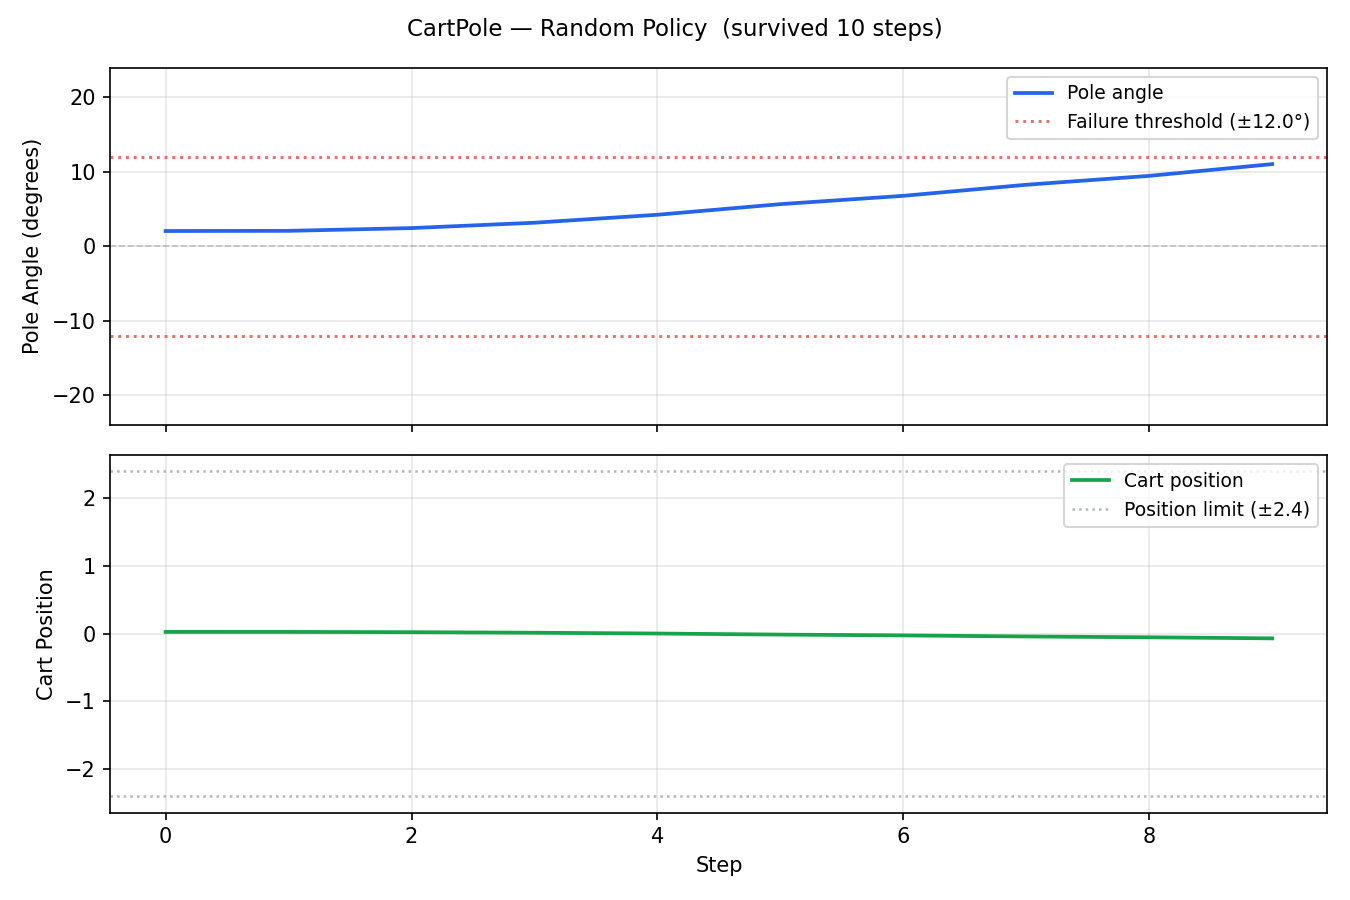
\includegraphics[width=\textwidth]{../results/task2/initial/control.png}
    \caption{Random policy: pole falls in $\approx$10 steps}
\end{subfigure}
\hfill
\begin{subfigure}[b]{0.47\textwidth}
    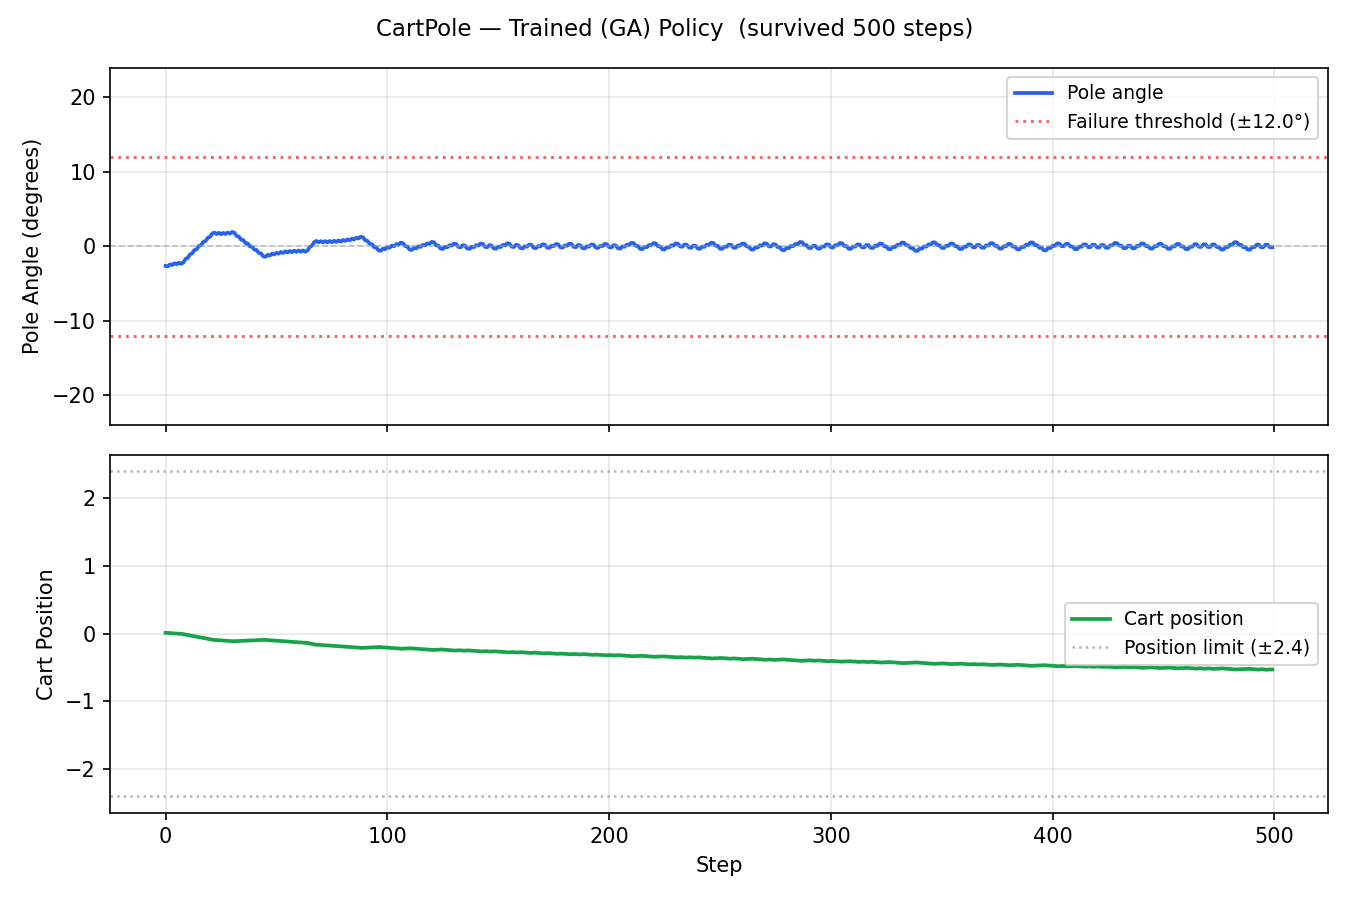
\includegraphics[width=\textwidth]{../results/task2/trained/control.png}
    \caption{Trained GA policy: 500 steps, angle near~$0^{\circ}$}
\end{subfigure}
\caption{CartPole control performance: before and after GA training}
\label{fig:cp_control}
\end{figure}

Figure~\ref{fig:cp_comparison} shows the side-by-side control comparison plot.

\begin{figure}[H]
\centering
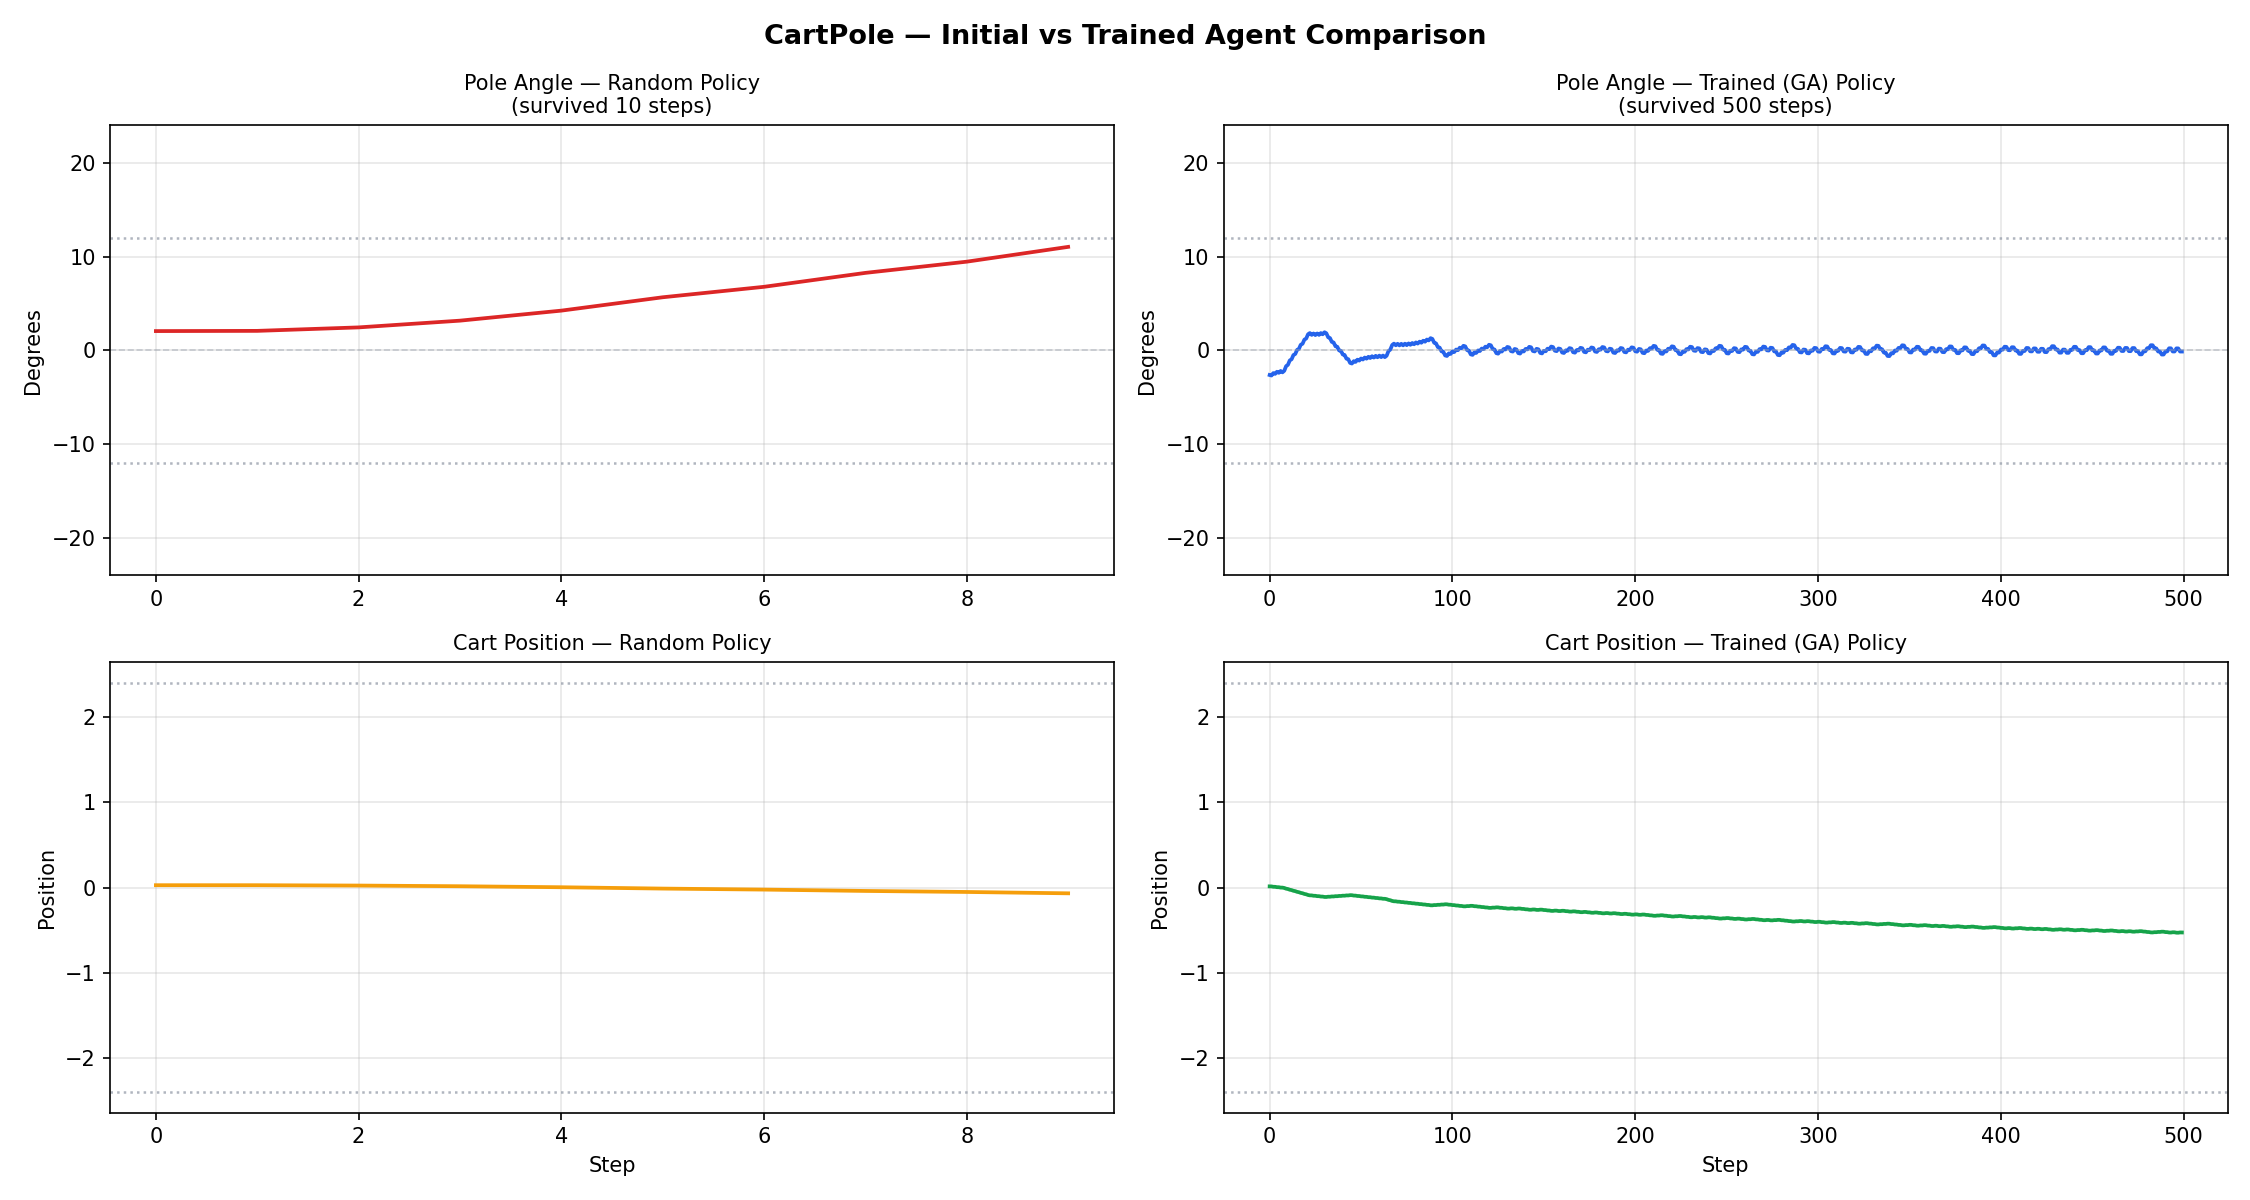
\includegraphics[width=0.85\textwidth]{../results/task2/comparison/control_comparison.png}
\caption{CartPole 2$\times$2 comparison: random policy (left column) vs trained policy (right column). Top row: pole angle with $\pm12^{\circ}$ failure thresholds. Bottom row: cart position with $\pm2.4$ position limits.}
\label{fig:cp_comparison}
\end{figure}

Figure~\ref{fig:cp_history} shows the reward history over training.

\begin{figure}[H]
\centering

\includegraphics[width=0.78\textwidth]{reward_history.png}
\caption{CartPole reward over 100 generations. Maximum reward of 500 is reached at generation 10. The dashed red line marks the episode length cap.}
\label{fig:cp_history}
\end{figure}

\subsection{Hyperparameter Experiments}

\subsubsection{Mutation Strength ($\sigma$)}

Figure~\ref{fig:cp_sigma} compares $\sigma \in \{0.05, 0.30, 1.00\}$.

\begin{figure}[H]
\centering
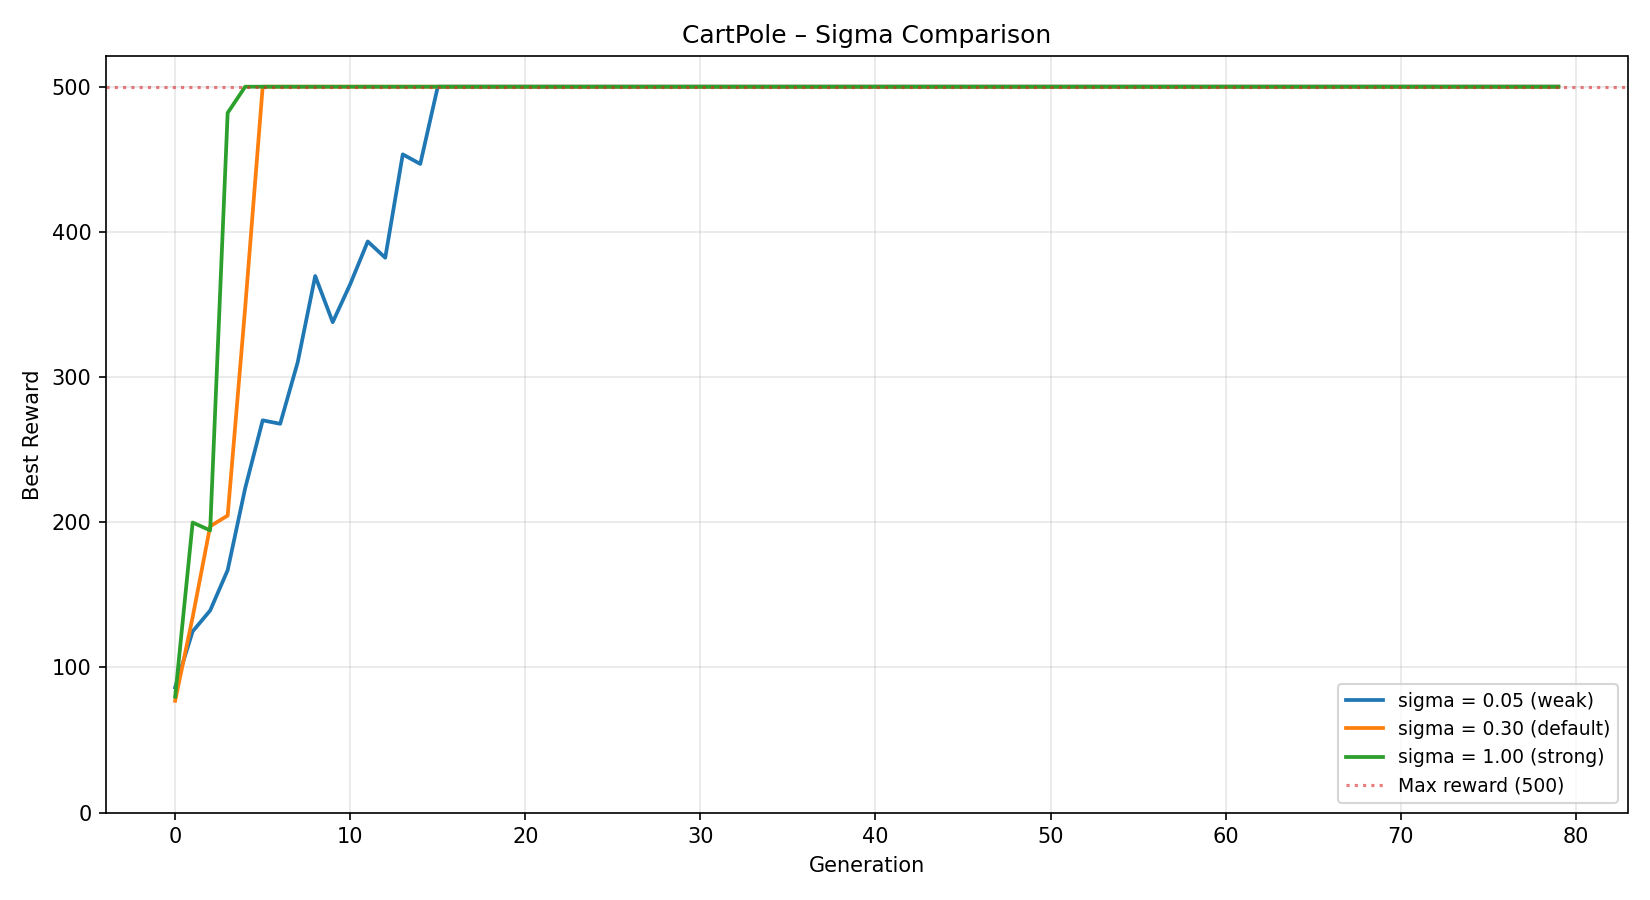
\includegraphics[width=0.80\textwidth]{comparison_sigma.png}
\caption{CartPole sigma comparison. All values eventually reach reward 500. Smaller $\sigma$ converges more smoothly; larger $\sigma$ shows higher initial variance but can escape local optima faster.}
\label{fig:cp_sigma}
\end{figure}

\subsubsection{Population Size}

Figure~\ref{fig:cp_pop} compares $n_\text{pop} \in \{20, 50, 100\}$.

\begin{figure}[H]
\centering

\includegraphics[width=0.80\textwidth]{comparison_population_size.png}
\caption{CartPole population size comparison. Larger populations start with better initial diversity: with pop=100, many individuals start near reward 500 by chance.}
\label{fig:cp_pop}
\end{figure}

\subsubsection{Evaluation Episodes}

Figure~\ref{fig:cp_eps} compares $n_\text{eval} \in \{1, 3, 5\}$.

\begin{figure}[H]
\centering
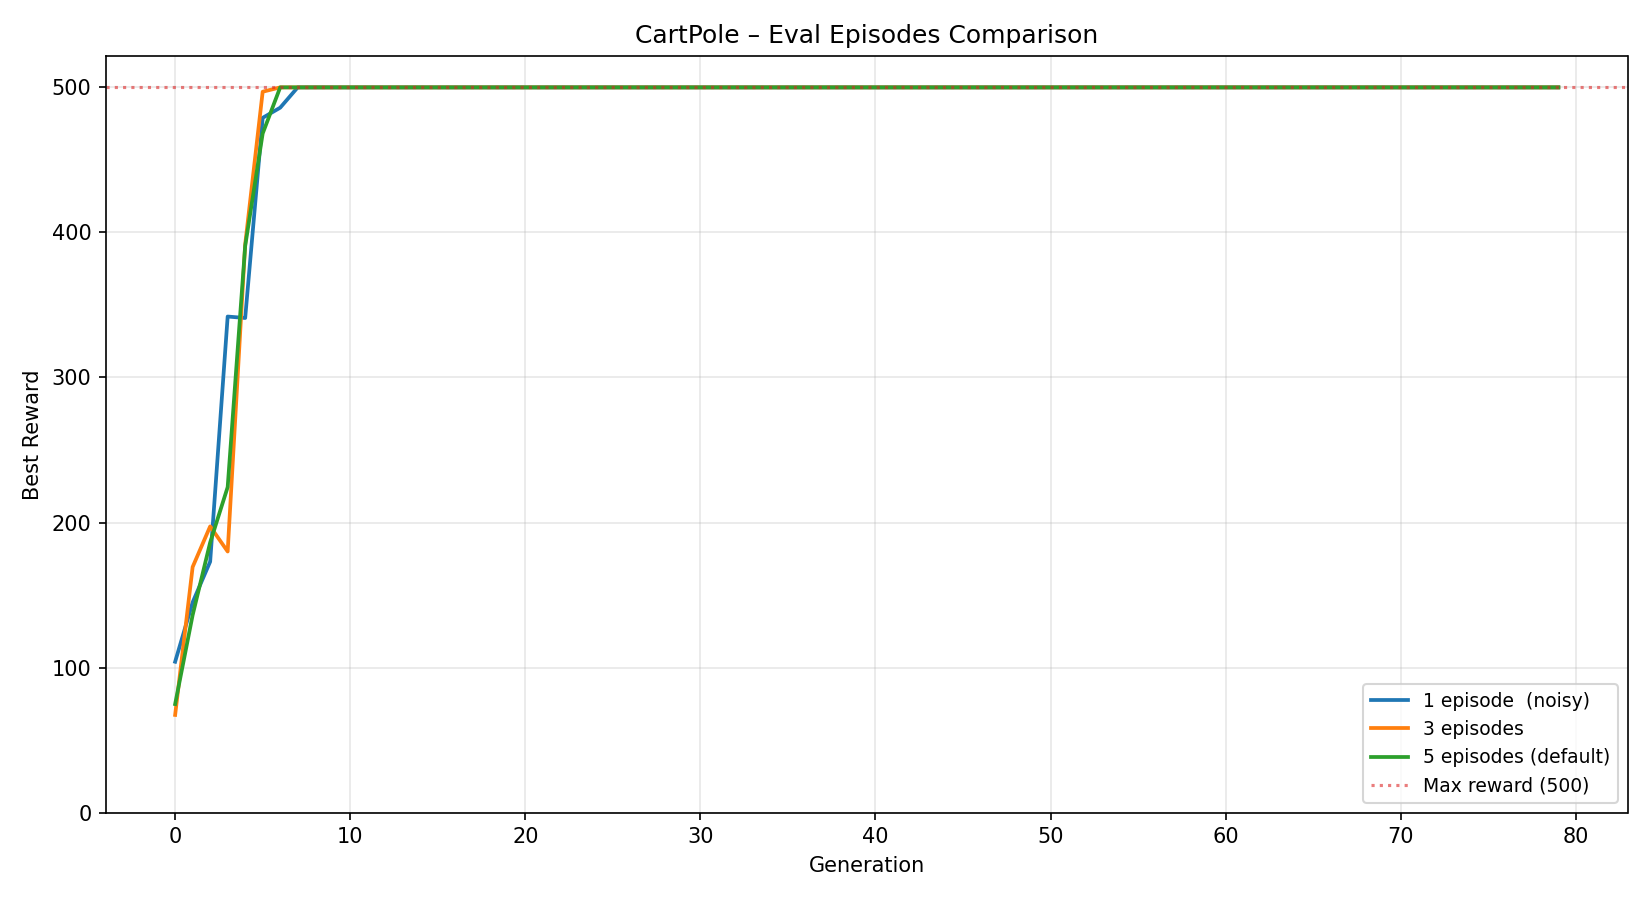
\includegraphics[width=0.80\textwidth]{comparison_eval_episodes.png}
\caption{CartPole evaluation episodes comparison. More episodes reduce fitness noise and produce smoother convergence curves, at the cost of more environment steps per generation.}
\label{fig:cp_eps}
\end{figure}

% ─────────────────────────────────────────────────────────────────────────────
\section{Improvements Following Reviewer Feedback}
\label{sec:improvements}
% ─────────────────────────────────────────────────────────────────────────────

The project was developed iteratively in response to two rounds of reviewer feedback.

\subsection{Feedback 1 (13 May 2026)}

\paragraph{Combined fitness functions.}
The original TSP fitness was the plain inverse distance. Following feedback, a path-balance (smoothness) bonus was added (Equation~\ref{eq:tsp_fitness}). The CartPole fitness was extended with a stability penalty (Equation~\ref{eq:cartpole_fitness}).

\paragraph{Parallel population evaluation.}
Fitness evaluation was parallelised using \texttt{ThreadPoolExecutor}. On an 8-core machine, this reduces CartPole training time by approximately $4\times$.

\paragraph{RL-inspired adaptive mutation.}
An adaptive boost mechanism was added: when fitness does not improve for \texttt{adaptive\_patience} consecutive generations, mutation is applied twice per offspring, doubling the exploration intensity.

\paragraph{Enhanced visualisations.}
The TSP fitness history plot was extended with a secondary y-axis showing route distance. A new control-performance plot was added for CartPole, showing pole angle and cart position over one episode.

\subsection{Feedback 2 (27 May 2026)}

\paragraph{Initial-state visualisation.}
Before running the GA, both tasks now record and visualise the initial (random) state: a random TSP route and a CartPole episode with random weights. This establishes a clear baseline for comparing before/after results.

\paragraph{Structured output folders.}
CartPole results are now organised into \texttt{initial/}, \texttt{trained/}, and \texttt{comparison/} subdirectories. Side-by-side comparison plots (2×2 grid) and a split-screen comparison video are generated automatically.

% ─────────────────────────────────────────────────────────────────────────────
\section{Experiments and Hyperparameter Analysis}
\label{sec:experiments}
% ─────────────────────────────────────────────────────────────────────────────

\subsection{Summary of Findings}

Table~\ref{tab:results} summarises the key numerical results.

\begin{table}[H]
\centering
\caption{Summary of experimental results}
\label{tab:results}
\begin{tabular}{lccl}
\toprule
\textbf{Task} & \textbf{Metric} & \textbf{Value} & \textbf{Notes} \\
\midrule
TSP & Best distance & 3.43 & Theoretical optimum $\approx$ 3.1 (10\% gap) \\
TSP & Initial distance & $\approx$ 6--8 & Random permutation \\
CartPole & Best reward & 500 / 500 & Maximum possible \\
CartPole & Convergence gen. & 10 & Out of 100 total \\
\bottomrule
\end{tabular}
\end{table}

\subsection{TSP Operator Comparison}

All four tested operator combinations (swap+OX, inversion+OX, scramble+OX, inversion+PMX) converge to distances within 2\% of each other after 200 generations. This suggests that for 20-city TSP, the choice of crossover or mutation operator has a smaller effect than population size or number of generations. For larger instances, the gap between OX and PMX would likely widen.

\subsection{CartPole Convergence Speed}

CartPole-v1 is considered solved (mean reward $\geq 475$ over 100 consecutive episodes). In our experiments, the best individual consistently achieves reward 500 within 10--15 generations regardless of hyperparameters, indicating that the linear policy space has a relatively simple fitness landscape for this problem. The main effect of hyperparameter choices (sigma, population size, evaluation episodes) is on the \emph{smoothness} of the convergence curve rather than the final quality.

% ─────────────────────────────────────────────────────────────────────────────
\section{Conclusions}
\label{sec:conclusions}
% ─────────────────────────────────────────────────────────────────────────────

This project demonstrated that a single, well-designed genetic algorithm framework can solve fundamentally different optimisation problems — a discrete combinatorial problem (TSP) and a continuous control problem (CartPole) — by parameterising all domain-specific logic through a five-callable plugin interface.

\paragraph{Key results.}
\begin{itemize}
    \item TSP: GA reduces the route distance from a random baseline of~6--8 to~\textbf{3.43}, within~10\% of the theoretical optimum for 20~cities.
    \item CartPole: GA discovers a functional linear controller in as few as~\textbf{10 generations}, achieving the maximum episode reward of~500 consistently.
\end{itemize}

\paragraph{Architectural contribution.}
The plugin interface (Section~\ref{sec:arch}) is the primary architectural contribution. It allows any new optimisation problem to be plugged into the framework by implementing five functions, with zero changes to \texttt{ga\_base.py}. This design pattern (dependency injection) is common in professional software but rarely emphasised in introductory GA implementations.

\paragraph{Future work.}
\begin{itemize}
    \item \textbf{MLP policy for CartPole}: A small neural network ($4 \to 8 \to 1$ architecture, 41 parameters) could be explored as an extension. The chromosome would be a flat weight vector; the framework requires only a new \texttt{init\_fn} and \texttt{fitness\_fn}.
    \item \textbf{Larger TSP instances}: Testing on 50--100 cities would reveal more pronounced differences between OX and PMX crossover.
    \item \textbf{Other Gymnasium environments}: LunarLander-v2 or BipedalWalker would test the framework on higher-dimensional continuous control.
    \item \textbf{Island model}: Running multiple independent populations and periodically exchanging best individuals could improve diversity and final solution quality.
\end{itemize}

% ─────────────────────────────────────────────────────────────────────────────
\section*{Appendix: Running the Code}
% ─────────────────────────────────────────────────────────────────────────────

\begin{lstlisting}[language=bash, caption={Setup and execution}]
# Setup
python3 -m venv .venv && source .venv/bin/activate
pip install -r requirements.txt

# Task 1 - TSP
python3 -m src.task1_tsp.tsp_ga          # train + visualise
python3 -m src.task1_tsp.experiments     # hyperparameter sweep

# Task 2 - CartPole
python3 -m src.task2_cartpole.train_ga   # train + record videos
python3 -m src.task2_cartpole.evaluate   # evaluate best agent
python3 -m src.task2_cartpole.experiments
\end{lstlisting}

% ─────────────────────────────────────────────────────────────────────────────
\begin{thebibliography}{9}

\bibitem{holland1975}
Holland, J.H. (1975). \textit{Adaptation in Natural and Artificial Systems}. University of Michigan Press.

\bibitem{goldberg1989}
Goldberg, D.E. (1989). \textit{Genetic Algorithms in Search, Optimisation and Machine Learning}. Addison-Wesley.

\bibitem{gymnasium2023}
Farama Foundation. (2023). Gymnasium: A Standard Interface for Reinforcement Learning Environments. \url{https://gymnasium.farama.org}.

\bibitem{ogata2010}
Ogata, K. (2010). \textit{Modern Control Engineering} (5th ed.). Prentice Hall.

\bibitem{numpy2020}
Harris, C.R., et al. (2020). Array programming with NumPy. \textit{Nature}, 585, 357--362.

\bibitem{imageio}
Klein, A., et al. (2023). imageio: Python library for reading and writing image data. \url{https://imageio.readthedocs.io}.

\end{thebibliography}

\end{document}
